\begin{frame}\frametitle{Long Baseline Neutrino Facility (LBNF). \\ Future Experiment (start in ~2022)}
\scriptsize
\begin{figure}
\label{fig:LBNF_overallScheme}
\centering
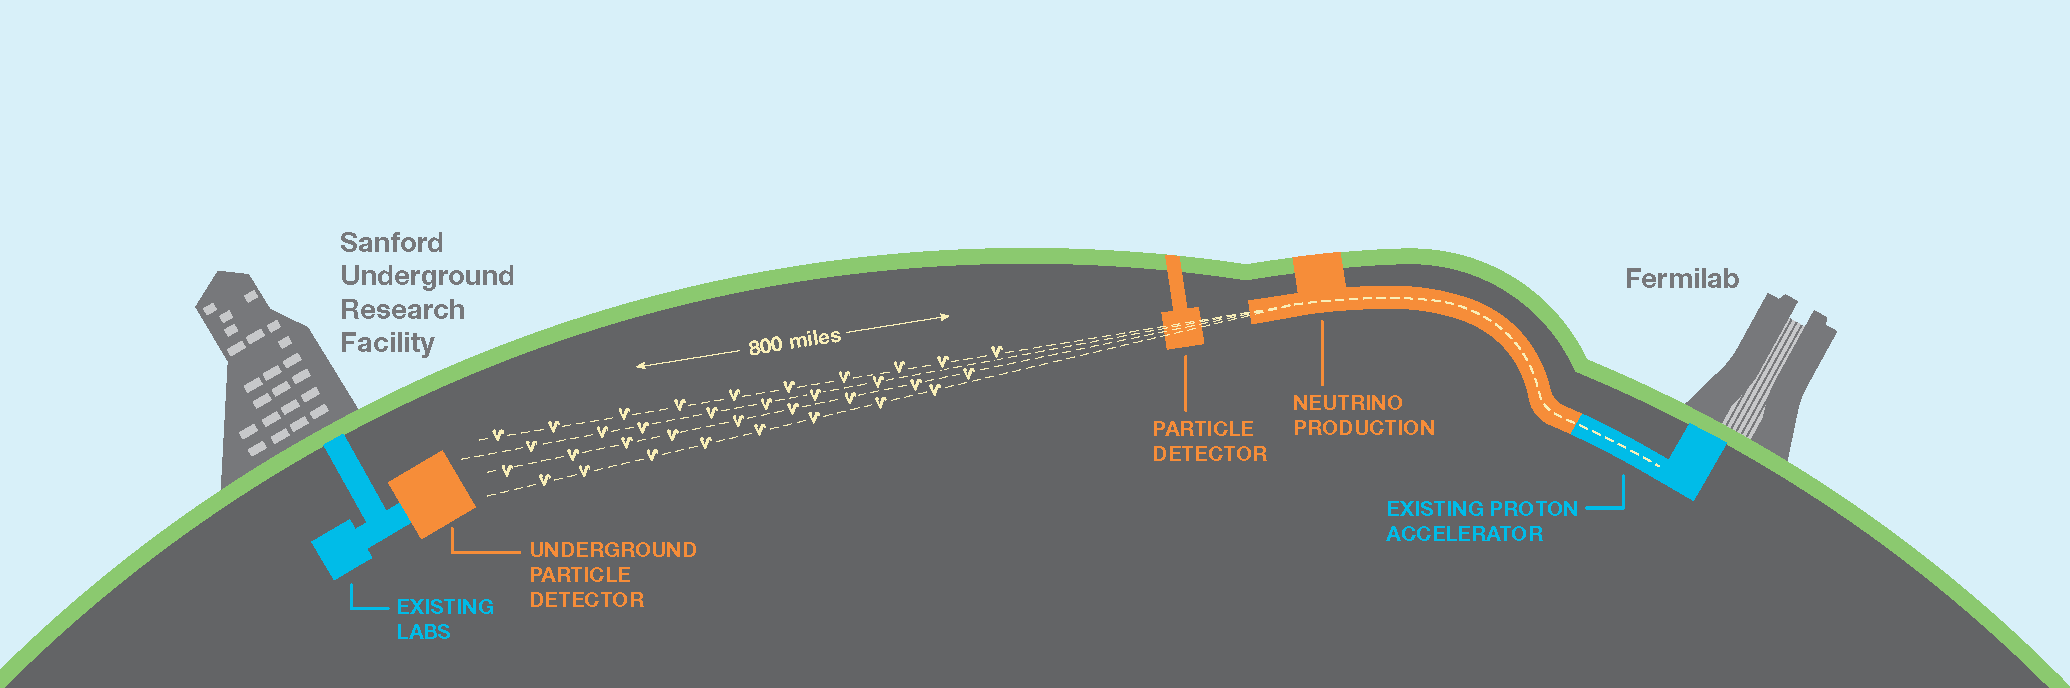
\includegraphics[width=0.85\textwidth, keepaspectratio=true]{figs/LBNF_overallScheme.png} 
\end{figure}
Plans to measure:
\begin{itemize}
     \item $\theta_{12}$, $\theta_{23}$, $\theta_{13}$, $|\Delta{m_{12}}^2|$, $|\Delta{m_{31}}^2|$
     \item CP-violation phase $\delta_{CP}$ and $\nu$ mass hierarchy (which never was measured before)
\end{itemize}
Experimental setup includes:  
\begin{itemize}
  \item neutrino beam production system at FNAL, Illinois 
  \item near detector at FNAL, Illinois 
  \item far detector at SURF, South Dakota
\end{itemize}
\tiny
"long baseline" - means neutrinos are likely to oscillate while travel from beam production system to the Far Detector. Short baseline - means neutrinos are unlikely to oscillate at such distance and appear at the detector as they are produced. Near detector performs short baseline measurements\\
FNAL - Fermilab National Accelerator Laboratory, SURF - Sanford Underground Research Facility\\
Source of figure: \cite{ref_LBNFweb} 
\end{frame}

\begin{frame}\frametitle{$P(\nu_\mu \rightarrow \nu_e)$ at a baseline of 1300 km}
  \scriptsize
  \begin{figure}
  \label{fig:LBNF_oscProbability}
  \centering
  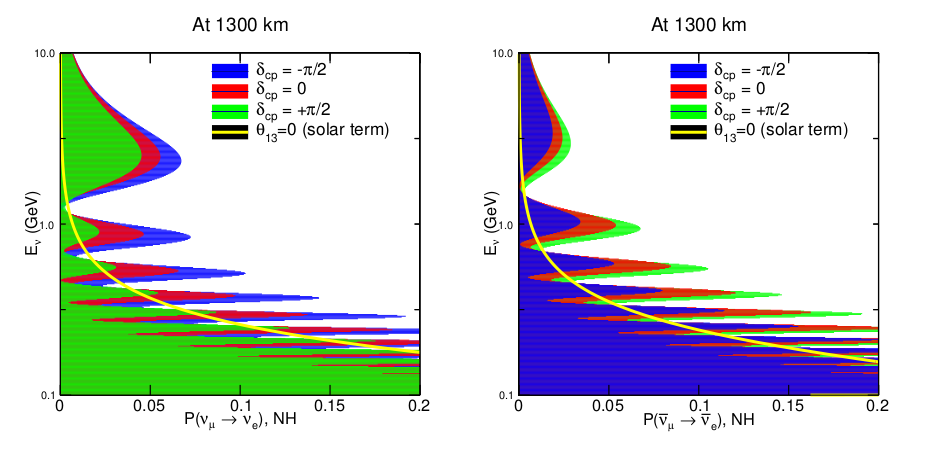
\includegraphics[width=0.98\textwidth, keepaspectratio=true]{figs/LBNF_oscProbability.png}
  \\$P(\nu_\mu \rightarrow \nu_e)$ at a baseline of 1300 km (as LBNF will have), as a function of neutrino energy. Left - neutrinos, right - antineutrinos. Source of figure: LBNF CDR draft, volume physics \cite{ref_LBNFdoc_volume-physics}
  \end{figure}
\end{frame}

\begin{frame}\frametitle{LBNF. Beam Production System}
\scriptsize
\begin{figure}
\label{fig:LBNF_nuBeam}
\centering
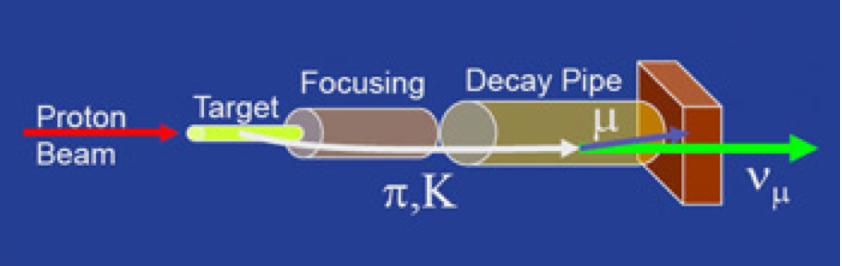
\includegraphics[width=0.65\textwidth, keepaspectratio=true]{figs/LBNF_nuBeam.png}  
\end{figure}
The neutrino beam production at the LBNF. Source of figure: \cite{ref_LBNFweb}\\
\begin{itemize}
  \item Proton beam from Fermilab accelerator hits target ($6.5\cdot10^{20}$ protons on target per year \cite{ref_LBNF_CDR_volumeBeam})
  \item Protons scatter on target atoms and produce pions and kaons {\tiny (more details on the next slide)}
  \item Charged pions and kaons are focused
  \item And decay in the decay pipe, producing muon neutrino beam
  \item Neutrinos are registered by near detector, $\sim 200$ m away from the target
  \item And by far detector, $\sim 1300$ km away from the target
\end{itemize}
Source of figure: \cite{ref_LBNFweb} 
\end{frame}

\begin{frame}\frametitle{LBNF. Feynmann diagrams of pions and kaons production and decay}
\scriptsize
\begin{figure}
\label{fig:pionAndKaonProductions}
\centering
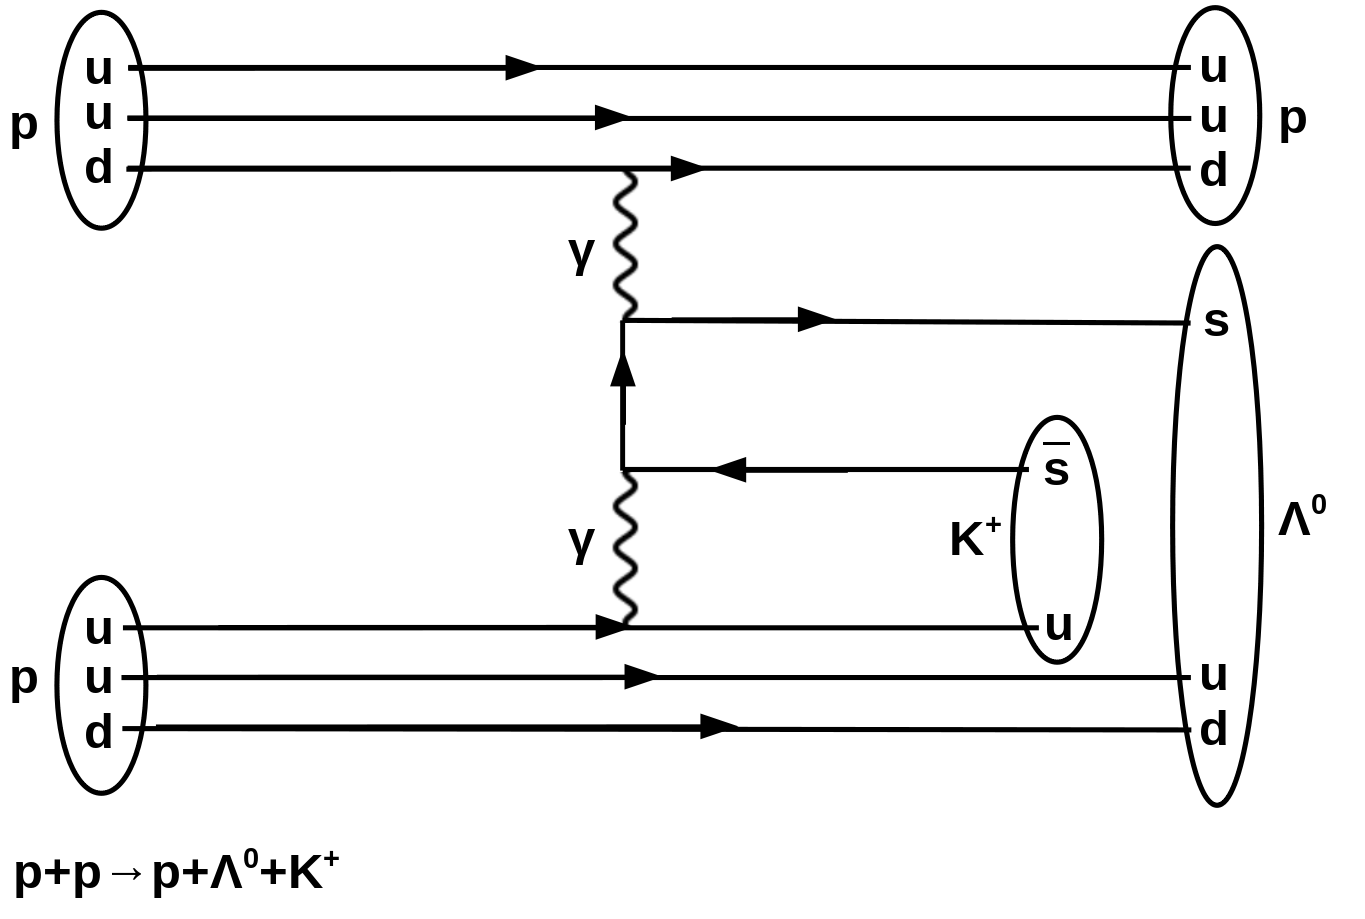
\includegraphics[width=0.48\textwidth, keepaspectratio=true]{figs/ppKaonProduction.png}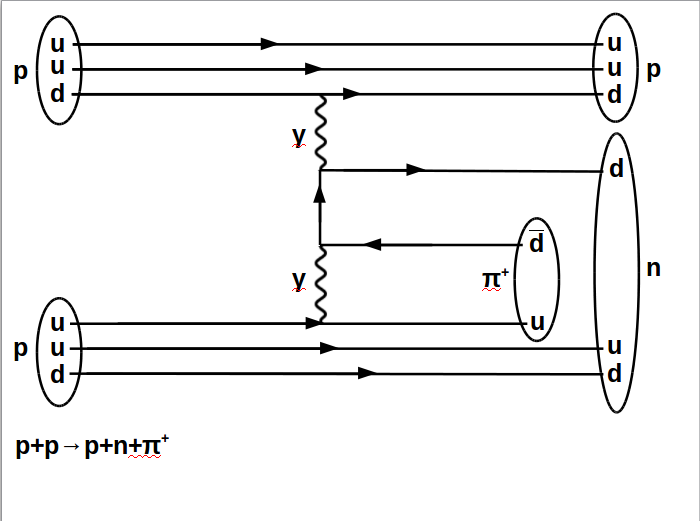
\includegraphics[width=0.48\textwidth, keepaspectratio=true]{figs/ppPionProduction.png}  
\end{figure}
\begin{figure}
\label{fig:pionAndKaonDecays}
\centering
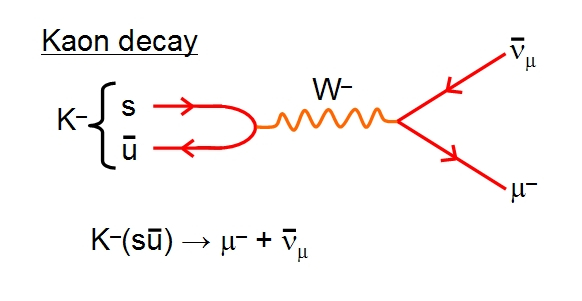
\includegraphics[width=0.45\textwidth, keepaspectratio=true]{figs/kaonDecay.jpg}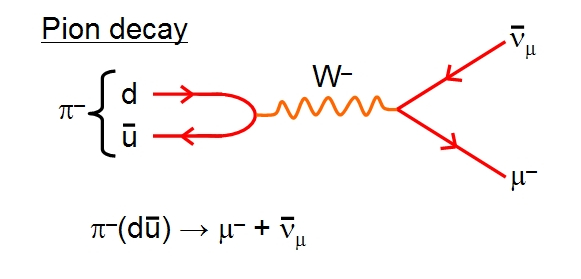
\includegraphics[width=0.45\textwidth, keepaspectratio=true]{figs/pionDecay.jpg} 
\end{figure}
\tiny Source of bottom figure \cite{ref_fig_pionandKaonDecays}.
\end{frame}

\begin{frame}\frametitle{LBNF. Expected $\nu$ and $\bar{\nu}$ Fluxes in Absence of Oscillations}
\begin{figure}
\centering
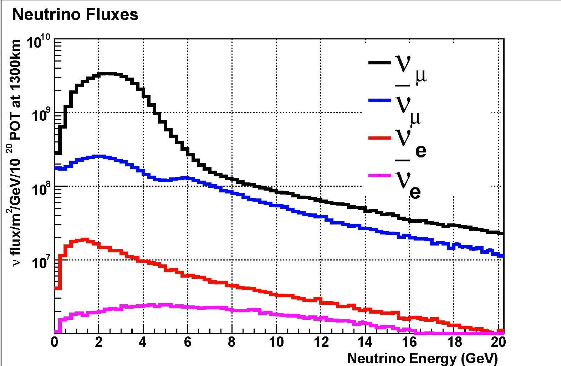
\includegraphics[width=0.48\textwidth, keepaspectratio=true]{figs/LBNF_nuFlux01.png}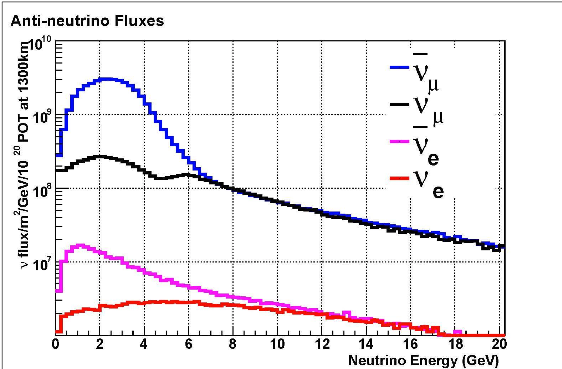
\includegraphics[width=0.48\textwidth, keepaspectratio=true]{figs/LBNF_nuFlux02.png}  
\end{figure}
\scriptsize
"POT" means \# of protons on the target\\
for LBNF beam: $6.5\cdot10^{20}$ POT per year expected\\
\tiny
Source of figure: \cite{ref_LBNF_CDR_volumeBeam}
\end{frame}

\begin{frame}\frametitle{LBNF. Near Detector Cavern}

\begin{columns} % contents are top vertically aligned
     \begin{column}{5cm} % each column can also be its own environment
     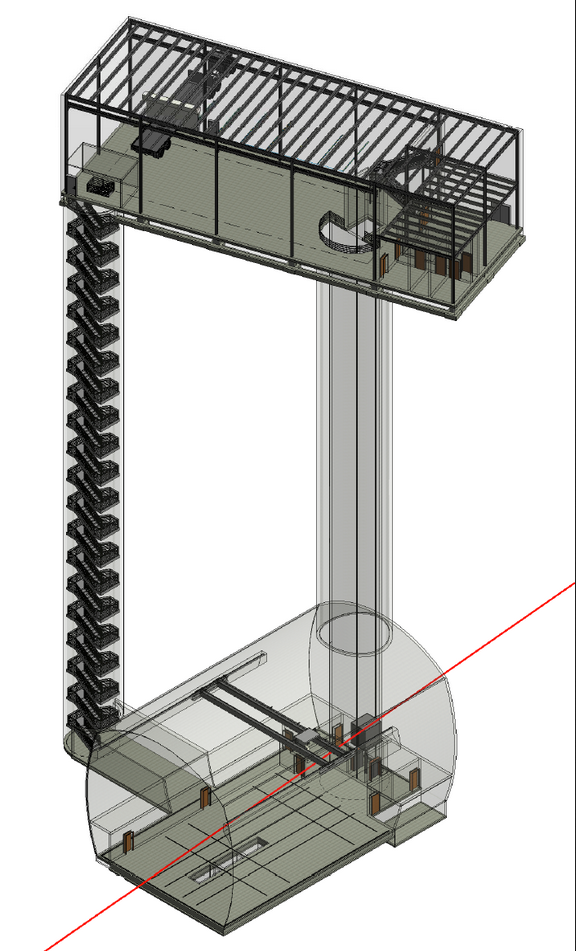
\includegraphics[width=0.80\textwidth, keepaspectratio=true]{figs/nearDetector_project.png}\\
     \tiny Source of figure: \cite{ref_LBNFweb} 
     \end{column}
     \begin{column}{5cm} % alternative top-align that's better for graphics
       \scriptsize
       Deep Underground Neutrino Experiment (DUNE)
Quoting the LBNF website \cite{ref_LBNFweb}, "The DUNE near detector will require LBNF to excavate and provision a cavern 200 ft (60 m) below grade on the Fermilab site and to construct a surface building directly above it. An elevator will provide the primary access between the two spaces; the stairway shown is planned for emergency egress. This complex will be constructed a minimum of 690 feet (210 m) downstream of the beamline target."   
     \end{column}
\end{columns}
\end{frame}

\begin{frame}\frametitle{LBNF. Near Detector}
\scriptsize
\begin{figure}
\label{fig:nearDetector}
\centering
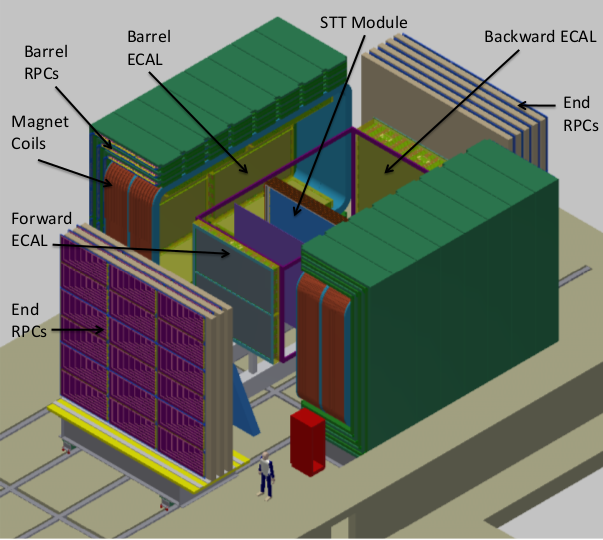
\includegraphics[width=0.50\textwidth, keepaspectratio=true]{figs/nearDetector.png}
\end{figure}
\scriptsize
The detector will consist of central Straw-Tube Tracker (STT) modules (neutrino targets will be built into the tracker), electromagnetic calorimeter (ECAL), magnet coils of 0.4T and muon identification system consisting of Resistive Plate Chamber (RPC) modules. The neutrinos would come from the bottom left corner of the picture, to the End RPCs.\\
\tiny
Source of figure: \cite{ref_LBNFdoc_volume-detectors}
\end{frame}

\begin{frame}\frametitle{LBNF. Near Detector Targets}
\scriptsize
\begin{figure}
\centering
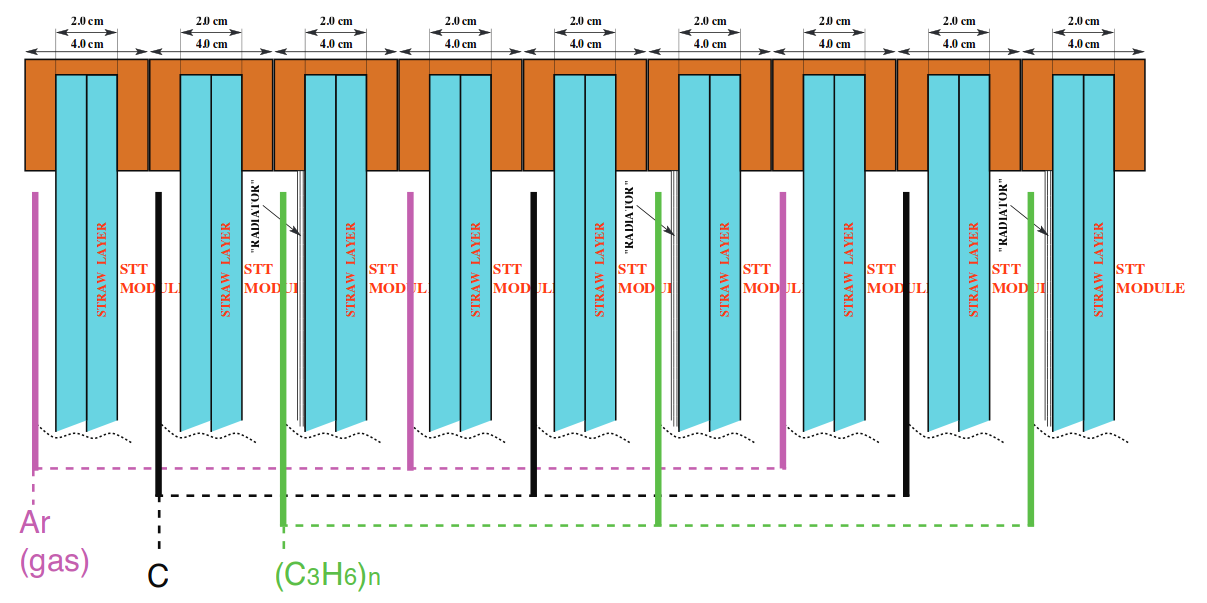
\includegraphics[width=0.95\textwidth, keepaspectratio=true]{figs/nearDetector_targetsMain.png}
\end{figure}
\scriptsize
Targets mounted inside the Straw-Tube Tracker to perform Near Detector neutrino physics measurements 
\begin{itemize}
  \item pressured Ar(gas)
  \item $(C_3H_6)_n$ radiators
  \item C(graphite)
\end{itemize}
\tiny
Source of figure: presentation "Nuclear Targets and Precision Measurements in DUNE ND" by R. Petti at \cite{ref_LBNF_collaborationMeeting}
\end{frame}


\begin{frame}\frametitle{LBNF. SURF (Far Detector Site)}
\begin{figure}
\label{fig:farDetector_SURF1}
\centering
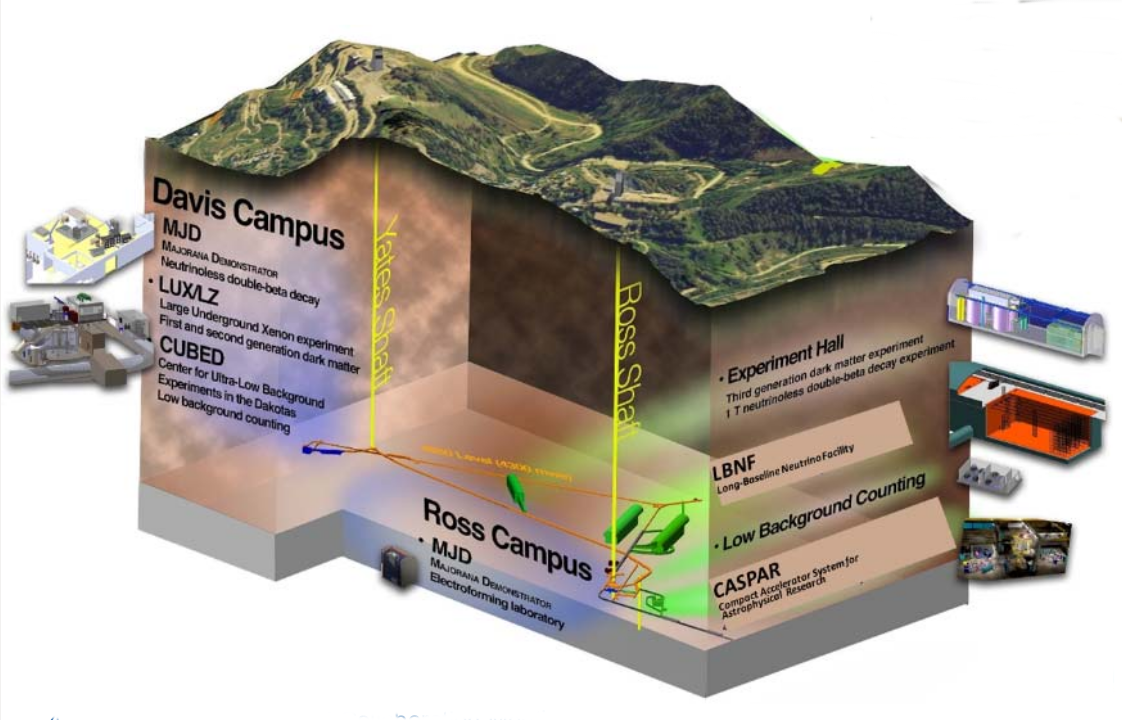
\includegraphics[width=0.98\textwidth, keepaspectratio=true]{figs/farDetector_SanfordUndergroundResearchFacility.png}
\tiny Source of figure: \cite{ref_LBNF_collaborationMeeting}
\end{figure}

\end{frame}

\begin{frame}\frametitle{LBNF. SURF (Far Detector Site)}
\begin{figure}
\label{fig:farDetector_SURF2}
\centering
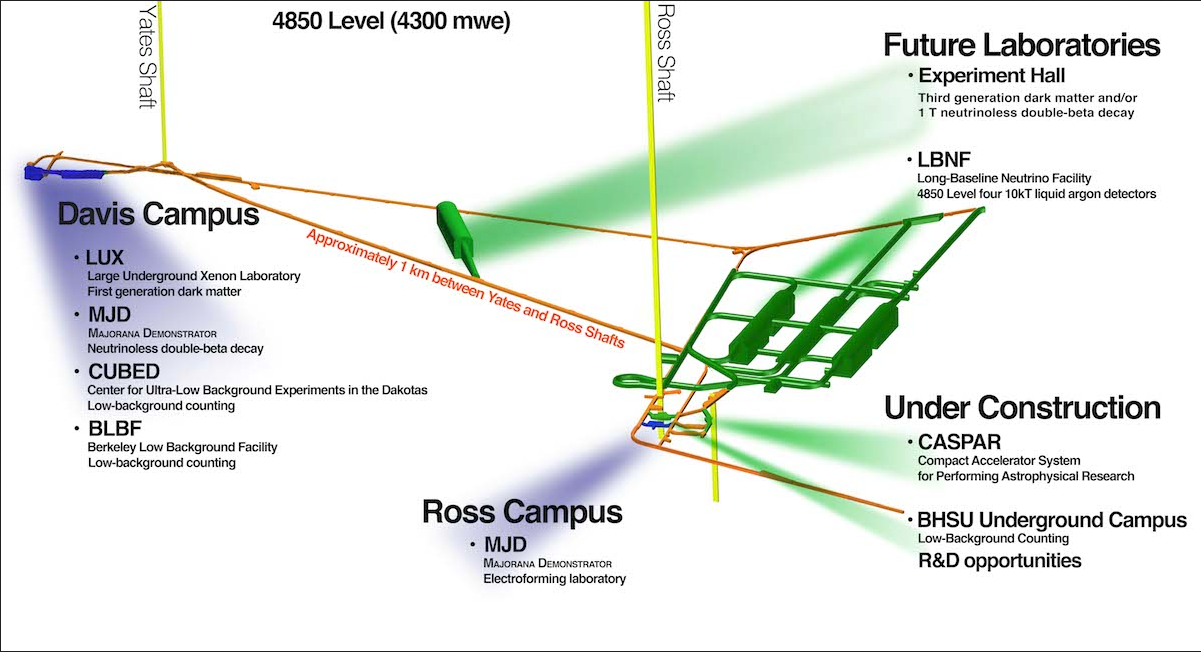
\includegraphics[width=0.98\textwidth, keepaspectratio=true]{figs/farDetector_wholeLab.png}
\end{figure}
\scriptsize
4 modules (15m x 12m x 58m, 10,000 tonnes of liquid argon each) placed into 4 caverns 1500 m underground. 5th cavern between two pairs - cryogenic equipment  \cite{ref_LBNFweb} \\
\end{frame}

\begin{frame}\frametitle{LBNF. Far Detector. Liquid Argon Time Projection Chamber}
\begin{figure}
\label{fig:farDetector_TPC}
\centering
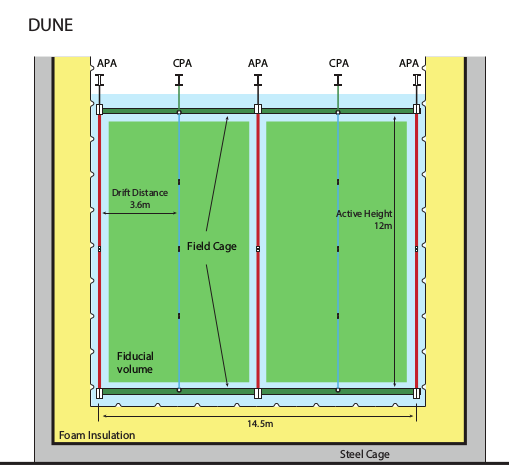
\includegraphics[width=0.70\textwidth, keepaspectratio=true]{figs/farDetector_TPC.png}
\end{figure}
\tiny
Source of figure: \cite{ref_LBNFdoc_volume-detectors}
\end{frame}

\begin{frame}\frametitle{LBNF Compared to the Other Experiments \cite{ref_LBN_OscExpReview}}
\tiny
\centering
  \begin{tabular}{|c|c|c|c|c|c|}
              & KEK (K2K) & NuMI & CNGS & T2K & LBNF (DUNE)\\ \hline
     location & Japan  & Illinois - & Switzerland - & Japan & Illinois - \\ 
              &        & Minnesota & Italy &  & South Dakota\\ \hline
     accelerator & KEK PS  & FNAL & CERN's SPS & J-PARC & FNAL\\ \hline
     time of oper. & 1999-2004  & 2005-2012 & 2006-2012 & 2010- & future \\ \hline 
     beam power  &  5 kW  & 300-350 kW  & 300 kW & 750 kW & 2000 kW\\ \hline 
     $E_p$  & 12 GeV & 120 GeV & 400 GeV & 30 GeV & 60-120 GeV\\ \hline 
     baseline  & 250 km & 735 km & 730 km & 295 km & 1300 km\\ \hline 
%                & KEK (K2K)   & NuMI                & CNGS                & T2K         & LBNF (DUNE)\\ \hline
     near        & (water ChD) & MINOS               & (muon               & ND280       & DUNE (FGD)\\  
     detector(s) & (FGD)       & (track. and scint.) & detector)           & INGRID      & \\ \hline 
%     ND mass     & 1 kt (ChD)  & 0.98 kt             &                     &             & \\ \hline 
     far         & SuperK      & MINOS               & ICARUS (LAr)        & SuperK      & DUNE (LAr)\\  
     detector(s) & (water ChD) & track. and scint.   & OPERA (FGD)        & (water ChD) & \\ \hline 
     FD mass     & 50 kt       & 5.4 kt              & 0.76 kt (ICARUS)   & 50 kt       & 40 kt\\ 
                 &             &                     & 1.25 kt (OPERA)    &             & \\ \hline 
 \end{tabular}
\end{frame}

\begin{frame}\frametitle{LBNF Summary}
  \scriptsize
  \begin{itemize}

     \item LBNF - long baseline neutrino oscillations experiment under development to be hosted by FNAL and SURF 
     \item Conceptual Design Report (CDR) drafts are partially available
     \item First collaboration meeting took place on April 16th-18th, 2015
     \item Collaboration of $>750$ people ($\sim$ 200 attended the 1st meeting on April 16th-18th of 2015)
     \item Expected parameters: baseline - 1300 km, beam power - 2 MW, far detector - 40kt of liquid argon
     \item Fermilab accelerator is available 
     \item Cavern for the near detector to be excavated
     \item Caverns for the far detector exist (former Homestake mine)
     \item plan: far detector installation in 2021-2022
     \item plan on precise measuments of $\theta_{12}$, $\theta_{23}$, $\theta_{13}$, $|\Delta{m_{12}}^2|$, $|\Delta{m_{31}}^2|$
     \item expected: to measure CP-violation phase $\delta_{CP}$ and $\nu$ mass hierarchy which never was measured before
     \item not expected: to measure absolute values of $\nu$ masses (different type of experiment would be needed)
  \end{itemize}
\end{frame}
